\documentclass[aspectratio=169]{beamer}

\usepackage{Archivo}
\renewcommand{\sfdefault}{\rmdefault}
\usepackage{graphicx}
\usepackage{tikz}
\usetikzlibrary{calc,positioning}
\tikzset{
  invisible/.style={opacity=0, text opacity=0},
  visible on/.style={alt={#1{}{invisible}}},
  alt/.code args={<#1>#2#3}{%
    \alt<#1>{\pgfkeysalso{#2}}{\pgfkeysalso{#3}}%
  },
}
\usepackage[most]{tcolorbox}
\usepackage{listings}

%% ---- Superteam Poland brand colors ----
\definecolor{stpldark}{HTML}{0B0E0F}   % near-black background
\definecolor{stplcard}{HTML}{161A1B}   % card / block surface
\definecolor{stplborder}{HTML}{1E2526}  % subtle track color for progress bar
\definecolor{stplred}{HTML}{DC143C}    % brand crimson red
\definecolor{stplwhite}{HTML}{FFFFFF}  % white
\definecolor{stplmuted}{HTML}{8A9BA8}  % muted / secondary text

\usetheme{default}
\setbeamersize{text margin left=0.85cm, text margin right=0.85cm}

%% ---- Background & base text ----
\setbeamercolor{background canvas}{bg=stpldark}
\setbeamercolor{normal text}{fg=stplwhite, bg=stpldark}
\usebeamercolor{normal text}

%% ---- Background image helpers ----
\newcommand{\stpldefaultbg}{%
  \setbeamertemplate{background}{%
    \begin{tikzpicture}[remember picture, overlay]
      \node[at=(current page.center), inner sep=0pt] {%
        \includegraphics[width=\paperwidth,height=\paperheight]{images/bg-default.png}%
      };
      \fill[stplborder]
        (current page.north west) rectangle
        ([yshift=-2.5pt]current page.north east);
      \pgfmathsetmacro{\stplprog}{\insertframenumber/\inserttotalframenumber}
      \fill[stplred]
        (current page.north west) rectangle
        ($(current page.north west)+(\stplprog\paperwidth,-2.5pt)$);
    \end{tikzpicture}%
  }%
}
\newcommand{\stplherobg}{%
  \setbeamertemplate{background}{%
    \includegraphics[width=\paperwidth,height=\paperheight]{images/bg-hero.png}%
  }%
}
\stpldefaultbg

%% ---- Structure ----
\setbeamercolor{structure}{fg=stplred}

%% ---- Title slide metadata ----
\setbeamercolor{title}{fg=stplwhite}
\setbeamercolor{subtitle}{fg=stplred}
\setbeamercolor{author}{fg=stplwhite}
\setbeamercolor{institute}{fg=stplmuted}
\setbeamercolor{date}{fg=stplmuted}

%% ---- Frame title: flat, no box background ----
\setbeamercolor{frametitle}{fg=stplwhite, bg=}
\setbeamerfont{frametitle}{size=\large, series=\bfseries}
\setbeamertemplate{frametitle}{%
  \vspace{0.35cm}%
  {\centering\insertframetitle\par}%
  \nointerlineskip\vspace{0.18cm}%
  \hfil{\color{stplred}\rule{2.2cm}{1.5pt}}\hfil\par%
}



%% ---- Incremental reveals ----
%% Bullets reveal one at a time by default. See style.md §4.5 for the two
%% per-frame opt-outs (static frame: `\begin{frame}<1>{...}`; manually
%% choreographed frame: `\beamerdefaultoverlayspecification{}` at frame top).
\beamerdefaultoverlayspecification{<+->}

%% ---- Bullet items ----
\setbeamercolor{itemize item}{fg=stplred}
\setbeamercolor{itemize subitem}{fg=stplmuted}
\setbeamercolor{itemize subsubitem}{fg=stplmuted}
\setbeamertemplate{itemize item}{\bfseries\textendash}
\setbeamertemplate{itemize subitem}{\small\textendash}
\setbeamercolor{enumerate item}{fg=stplred}
\setbeamercolor{enumerate subitem}{fg=stplmuted}
\setbeamertemplate{enumerate item}{\textcolor{stplred}{\bfseries\insertenumlabel.}}
\setbeamertemplate{enumerate subitem}{\textcolor{stplmuted}{\small\insertenumlabel.}}

%% ---- Blocks (flat left-accent via tcolorbox) ----
\tcbset{
  stplbase/.style={
    enhanced, breakable,
    colback=stplcard, coltext=stplwhite,
    coltitle=stplwhite, fonttitle=\bfseries,
    boxrule=0pt, leftrule=3pt,
    arc=0pt, outer arc=0pt,
    top=5pt, bottom=5pt, left=7pt, right=7pt,
    toptitle=4pt, bottomtitle=4pt,
    titlerule=0pt,
  },
}
\renewenvironment{block}[1]{%
  \pause%
  \begin{tcolorbox}[stplbase, colframe=stplred, title={#1}]%
}{%
  \end{tcolorbox}%
}
\renewenvironment{alertblock}[1]{%
  \pause%
  \begin{tcolorbox}[stplbase, colframe=stplred!75!black,
    colback=stplred!10!stplcard, title={#1}]%
}{%
  \end{tcolorbox}%
}
\renewenvironment{exampleblock}[1]{%
  \pause%
  \begin{tcolorbox}[stplbase, colframe=stplmuted, title={#1}]%
}{%
  \end{tcolorbox}%
}

%% ---- Code listings (Rust + Anchor) ----
\lstdefinelanguage{Rust}{
  keywords={fn,pub,struct,impl,trait,let,mut,self,Self,match,return,for,in,
            if,else,enum,use,mod,as,where,Option,Result,Some,None,Ok,Err,
            u8,u16,u32,u64,i64,u128,bool,String,Vec,Pubkey,Context,msg,vec,
            Account,Signer,Program,System,has_one,init,payer,space,seeds,bump},
  morecomment=[l]{//},
  morestring=[b]",
  sensitive=true,
}
\lstset{
  basicstyle=\ttfamily\scriptsize\color{stplwhite},
  backgroundcolor=\color{stplcard},
  keywordstyle=\color{stplred}\bfseries,
  commentstyle=\color{stplmuted},
  stringstyle=\color{stplmuted},
  showstringspaces=false,
  keepspaces=true,
  columns=fixed,
  basewidth=0.46em,
  frame=leftline,
  framerule=2pt,
  rulecolor=\color{stplred},
  xleftmargin=0.6em,
  aboveskip=0.4em,
  belowskip=0.2em,
  language=Rust,
  escapeinside={(*@}{@*)},
}

%% ---- Code reveal card (line-synced to bullets) ----
%% A block-styled card WITHOUT the block's auto-\pause, so it is visible from
%% the current overlay and its code lines can reveal in step with the itemize
%% bullets via (*@\onslide<k->@*) markers. The listing drops its own
%% background/frame (style=reveal) so the solid card shows through instead of
%% the per-line background going ragged as lines are covered.
\newtcolorbox{codeblock}[1]{stplbase, colframe=stplred, title={#1}}
\lstdefinestyle{reveal}{backgroundcolor={}, frame=none, xleftmargin=0pt,
  aboveskip=0pt, belowskip=0pt}

%% ---- Table of contents ----
\setbeamercolor{section in toc}{fg=stplwhite}
\setbeamercolor{subsection in toc}{fg=stplmuted}
\setbeamertemplate{section in toc}{%
  {\color{stplred}\textbf{\textendash}}\hspace{0.5em}\inserttocsection%
}

%% ---- Footline: minimal ----
%% Transparent bg so the background image shows through (normal text has
%% bg=stpldark, which would paint a flat band over the image's bottom glow).
\setbeamercolor{footline}{fg=stplwhite, bg=}
\setbeamertemplate{footline}{%
  \begin{beamercolorbox}[wd=\paperwidth, ht=0pt, dp=0.55cm]{footline}%
    \hspace{0.85cm}%
    \raisebox{-0.42cm}{\includegraphics[height=0.42cm]{images/stpl-logo.png}}%
    \hfill%
    \raisebox{-0.24cm}{\textcolor{stplmuted}{\tiny\insertframenumber\,/\,\inserttotalframenumber}}%
    \hspace{0.85cm}%
  \end{beamercolorbox}%
}
\setbeamertemplate{navigation symbols}{}

%% ---- Title page defaults (decks may override) ----
\date{\the\year}

%% ---- Title frame helper (uses hero background) ----
\newcommand{\maketitleframe}{%
  \stplherobg
  \begin{frame}[plain]%
    \titlepage%
  \end{frame}%
  \stpldefaultbg
}

%% ---- Section divider slides ----
\AtBeginSection[]{%
  \stplherobg
  \begin{frame}[plain]
    \begin{tikzpicture}[remember picture, overlay]
      \fill[stplred, opacity=0.07]
        ([xshift=-2.5cm]current page.east) circle (5.5cm);
      \fill[stplred]
        (current page.north west) rectangle ([xshift=5pt]current page.south west);
    \end{tikzpicture}%
    \vfill
    \hspace{0.1\paperwidth}%
    \begin{minipage}{0.8\paperwidth}
      \textcolor{stplmuted}{\small Section \thesection}\\[0.35cm]
      {\color{stplwhite}\LARGE\bfseries\insertsectionhead}\\[0.25cm]
      {\color{stplred}\rule{3cm}{1.5pt}}
    \end{minipage}%
    \vfill
  \end{frame}%
  \stpldefaultbg
}

%% ---- Title page ----
\setbeamertemplate{title page}{%
  \begin{tikzpicture}[remember picture, overlay]
    \fill[stplred]
      (current page.north west) rectangle ([xshift=5pt]current page.south west);
    \fill[stplred, opacity=0.07]
      ([xshift=-3cm,yshift=3cm]current page.north east) circle (5.5cm);
    \fill[stplred, opacity=0.04]
      ([yshift=-1.5cm]current page.south east) circle (3.5cm);
  \end{tikzpicture}%
  \vfill
  \hspace{0.08\paperwidth}%
  \begin{minipage}{0.85\paperwidth}
    \includegraphics[width=3cm]{images/stpl-logo.png}\par
    \vspace{0.8cm}
    {\usebeamerfont{title}\usebeamercolor[fg]{title}\inserttitle}\par
    \vspace{0.2cm}
    {\color{stplred}\rule{3cm}{1.5pt}}\par
    \vspace{0.3cm}
    {\usebeamerfont{subtitle}\usebeamercolor[fg]{subtitle}\insertsubtitle}\par
    \vspace{0.65cm}
    {\usebeamerfont{author}\usebeamercolor[fg]{author}\insertauthor}\par
    \vspace{0.12cm}
    {\small\textcolor{stplmuted}{\insertinstitute\enspace·\enspace\insertdate}}
  \end{minipage}%
  \vfill
}


\usepackage[utf8]{inputenc}
\usepackage[T1]{fontenc}

%% Deck-local listing keywords: CPI / PDA vocabulary absent from the shared
%% Anchor keyword set in preamble.tex.
\lstset{morekeywords={CpiContext,Interface,InterfaceAccount,TokenInterface,
                      TokenAccount,Mint,Token,TransferChecked,transfer_checked,
                      invoke_signed,new_with_signer,bumps,ProgramError,
                      derive,Accounts,is_signer,key,as_ref}}

\title{CPI i podpis PDA}
\subtitle{Program, który podpisuje --- Solana Bootcamp}
\author{}
\institute{Superteam Poland}

\begin{document}

\maketitleframe

\begin{frame}{Plan}
  \tableofcontents
\end{frame}

% ================================================================
\section{CPI}

% 1. Program nie ma rak --- problem hook (alertblock)
\begin{frame}{Program nie ma rąk}
  \begin{itemize}
    \item Z Lekcji 9: skarbiec programu to zwykłe konto tokenowe
    \item Z Lekcji 5: bajty konta zmienia wyłącznie jego program-właściciel
    \item Skarbiec należy do Token Programu --- nie do naszego programu
    \item To nie ograniczenie Anchora, tylko reguła samej sieci
  \end{itemize}
  \vspace{0.1cm}
  \begin{center}
    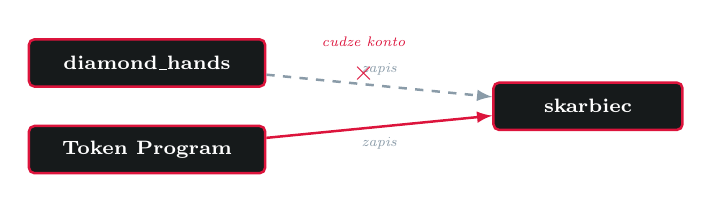
\begin{tikzpicture}[
        every node/.style={font=\scriptsize\bfseries, align=center},
        box/.style={
          draw=stplred, line width=0.9pt,
          fill=stplcard, text=stplwhite,
          rounded corners=2pt,
          minimum width=2.8cm, minimum height=0.6cm, align=center,
        },
        arr/.style={-latex, draw=stplred, line width=0.9pt},
        bad/.style={-latex, draw=stplmuted, line width=0.9pt, dashed},
        lbl/.style={font=\tiny\itshape, text=stplmuted},
      ]
      \node[box, minimum width=3.0cm] (d)  at (0,   0.48) {diamond\_hands};
      \node[box, minimum width=3.0cm] (tp) at (0,  -0.62) {Token Program};
      \node[box, minimum width=2.4cm] (v)  at (5.6, -0.07) {skarbiec};

      \draw[bad] (d) -- (v) node[midway, above, lbl] {zapis};
      \draw[arr] (tp) -- (v) node[midway, below, lbl] {zapis};

      % the crossed-out illegal write
      \node[font=\normalsize\bfseries, text=stplred] at (2.75, 0.34) {$\times$};
      \node[lbl, text=stplred] at (2.75, 0.75) {cudze konto};
    \end{tikzpicture}
  \end{center}
  \vspace{-0.05cm}
  \begin{alertblock}{Problem}
    Program ma wydać tokeny ze skarbca, ale nie wolno mu dotknąć konta,
    na którym one leżą.
  \end{alertblock}
\end{frame}

% 2. Cross-Program Invocation --- term debut (block: def)
\begin{frame}{Wywołanie programu}
  \begin{itemize}
    \item Skoro nie wolno pisać samemu --- trzeba poprosić właściciela
    \item Program w trakcie instrukcji wywołuje inny program
    \item To \textbf{Cross-Program Invocation (CPI)} --- z Lekcji 3 znane jako klocki
    \item Z Lekcji 6: atomowość obejmuje całe drzewo wywołań, nie jedną instrukcję
  \end{itemize}
  \vspace{0.1cm}
  \begin{center}
    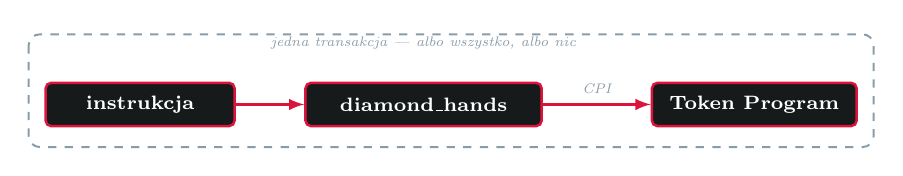
\begin{tikzpicture}[
        every node/.style={font=\scriptsize\bfseries, align=center},
        box/.style={
          draw=stplred, line width=0.9pt,
          fill=stplcard, text=stplwhite,
          rounded corners=2pt,
          minimum width=2.6cm, minimum height=0.55cm, align=center,
        },
        env/.style={draw=stplmuted, line width=0.7pt, dashed, rounded corners=4pt},
        arr/.style={-latex, draw=stplred, line width=0.9pt},
        lbl/.style={font=\tiny\itshape, text=stplmuted},
      ]
      \node[box, minimum width=2.4cm] (i)  at (0,   0) {instrukcja};
      \node[box, minimum width=3.0cm] (d)  at (3.6, 0) {diamond\_hands};
      \node[box, minimum width=2.6cm] (tp) at (7.8, 0) {Token Program};

      \draw[arr] (i) -- (d);
      \draw[arr] (d) -- (tp) node[midway, above, lbl] {CPI};

      \draw[env] ($(i.north west)+(-0.2,0.6)$) rectangle ($(tp.south east)+(0.2,-0.25)$);
      \node[lbl] at (3.6, 0.78) {jedna transakcja --- albo wszystko, albo nic};
    \end{tikzpicture}
  \end{center}
  \vspace{-0.05cm}
  \begin{block}{Definicja}
    CPI = instrukcja wywołana przez program, a nie przez użytkownika.
    Wywoływany program może w ten sam sposób wywołać kolejny.
  \end{block}
\end{frame}

% 3. CPI w Anchorze --- code IS the slide
\begin{frame}[fragile]{CPI w Anchorze}
  \begin{itemize}
    \item Najpierw struktura kont, których wymaga wywoływana instrukcja
    \item Potem kontekst: który program wywołać i z jakimi kontami
    \item \texttt{CpiContext::new} przyjmuje \textbf{program ID}, nie konto programu
    \item Na końcu wywołanie --- \texttt{decimals} czytane z mintu, nie wpisane na sztywno
  \end{itemize}
  \begin{codeblock}{Przelew ze skarbca użytkownika do programu}
\begin{lstlisting}[style=reveal]
(*@\onslide<1->@*)let cpi_accounts = TransferChecked {
(*@\onslide<1->@*)    from: ctx.accounts.payer_ata.to_account_info(),
(*@\onslide<1->@*)    to: ctx.accounts.vault.to_account_info(),
(*@\onslide<1->@*)    authority: ctx.accounts.payer.to_account_info(),
(*@\onslide<1->@*)    mint: ctx.accounts.mint.to_account_info(),
(*@\onslide<1->@*)};
(*@\onslide<3->@*)let cpi_ctx = CpiContext::new(
(*@\onslide<3->@*)    ctx.accounts.token_program.key(), cpi_accounts);
(*@\onslide<4->@*)transfer_checked(cpi_ctx, amount, ctx.accounts.mint.decimals)?;
\end{lstlisting}
  \end{codeblock}
\end{frame}

% 4. Ukryte CPI --- (exampleblock: cost illustration)
\begin{frame}{Ukryte CPI}
  \begin{itemize}
    \item Nie każde CPI widać w kodzie --- część dokłada sam Anchor
    \item \texttt{init} zleca Systemowi utworzenie konta i opłacenie rent
    \item Dla konta tokenowego dochodzi jeszcze inicjalizacja u Token Programu
  \end{itemize}
  \vspace{0.1cm}
  \begin{center}
    \begin{tikzpicture}[
        every node/.style={font=\scriptsize\bfseries, align=center},
        box/.style={
          draw=stplred, line width=0.9pt,
          fill=stplcard, text=stplwhite,
          rounded corners=2pt,
          minimum width=2.7cm, minimum height=0.5cm, align=center,
        },
        hid/.style={
          draw=stplmuted, line width=0.7pt,
          fill=stplcard, text=stplmuted,
          rounded corners=2pt,
          minimum width=3.2cm, minimum height=0.45cm, align=center,
          font=\tiny\bfseries,
        },
        arr/.style={-latex, draw=stplmuted, line width=0.7pt},
        mine/.style={-latex, draw=stplred, line width=0.9pt},
        lbl/.style={font=\tiny\itshape, text=stplmuted},
      ]
      \node[box, minimum width=2.2cm] (l) at (0, 0) {lockup};

      \node[hid] (c1) at (4.2,  0.95) {create\_account (locker)};
      \node[hid] (c2) at (4.2,  0.35) {create\_account (vault)};
      \node[hid] (c3) at (4.2, -0.25) {initialize\_account3};
      \node[box, minimum width=3.2cm] (c4) at (4.2, -0.9) {transfer\_checked};

      \draw[arr]  (l.east) -- (c1.west);
      \draw[arr]  (l.east) -- (c2.west);
      \draw[arr]  (l.east) -- (c3.west);
      \draw[mine] (l.east) -- (c4.west);

      \node[lbl] at (7.6,  0.35) {dokłada Anchor};
      \node[lbl, text=stplred] at (7.6, -0.9) {napisane ręcznie};
    \end{tikzpicture}
  \end{center}
  \vspace{-0.1cm}
  \begin{exampleblock}{Koszt}
    Każde z tych wywołań zużywa budżet obliczeniowy transakcji ---
    a w kodzie widać tylko ostatnie.
  \end{exampleblock}
\end{frame}

% 5. Ryzyka CPI --- (alertblock: arbitrary CPI)
\begin{frame}{Fałszywy program}
  \begin{itemize}
    \item Adres wywoływanego programu to zwykłe konto z transakcji
    \item Podstawiony program o tym samym interfejsie zrobi coś zupełnie innego
    \item Dlatego program ID musi być \textbf{przypięty}, a nie przyjęty od klienta
    \item \texttt{Program} i \texttt{Interface} odrzucają transakcję z obcym adresem
  \end{itemize}
  \vspace{0.15cm}
  \begin{alertblock}{Ryzyko}
    Wywołanie programu podanego przez użytkownika zamienia własny program
    w pośrednika dla cudzego kodu.
  \end{alertblock}
\end{frame}

% ================================================================
\section{PDA}

% 6. Podpis bez klucza --- problem hook (alertblock)
\begin{frame}{Podpis bez klucza}
  \begin{itemize}
    \item Przelew ze skarbca wymaga podpisu jego \texttt{authority}
    \item Gdyby authority miało klucz prywatny, ktoś musiałby go trzymać
    \item Kto trzyma klucz, ten opróżnia skarbiec --- wracamy do Lekcji 0
    \item Potrzebny adres, którego kluczem nie dysponuje nikt
  \end{itemize}
  \vspace{0.25cm}
  \begin{alertblock}{Sprzeczność}
    Skarbiec musi mieć authority, które podpisuje --- i jednocześnie nie może
    istnieć klucz zdolny go podpisać.
  \end{alertblock}
\end{frame}

% 7. Adres poza krzywa --- term debut (block: def)
\begin{frame}{Adres poza krzywą}
  \begin{itemize}
    \item Zwykły adres to klucz publiczny --- punkt na krzywej eliptycznej
    \item Adres można też policzyć: skrót z wybranych składników i ID programu
    \item Wynik celowo \textbf{nie leży} na krzywej --- nie ma do niego klucza prywatnego
    \item Taki adres to \textbf{Program Derived Address (PDA)}
  \end{itemize}
  \vspace{0.25cm}
  \begin{block}{Model myślowy}
    \texttt{PDA = h(ID programu + składniki)}. Składniki (\texttt{seeds}) wybiera
    autor programu --- np.\ słowo ,,vault'' i klucz użytkownika.
  \end{block}
\end{frame}

% 8. Bump --- term debut (block: def)
\begin{frame}{Bump}
  \begin{itemize}
    \item Skrót zwykle trafia \emph{na} krzywą --- czyli wynik jest bezużyteczny
    \item Do składników dokłada się wtedy jeden bajt i liczy ponownie
    \item Zaczyna się od 255 w dół; pierwszy \emph{poza} krzywą to \textbf{bump kanoniczny}
    \item Bump można zapisać w koncie albo szukać go przy każdym wywołaniu
  \end{itemize}
  \vspace{0.1cm}
  \begin{center}
    \begin{tikzpicture}[x=0.8cm, y=0.55cm,
        lbl/.style={font=\tiny\itshape, text=stplmuted},
      ]
      % Ed25519 curve, schematic: points on it have a private key
      \draw[draw=stplmuted, line width=0.8pt, smooth, samples=120, domain=-1.45:1.45]
        plot ({\x}, {sqrt(abs(1 - \x*\x))*1.15});
      \draw[draw=stplmuted, line width=0.8pt, smooth, samples=120, domain=-1.45:1.45]
        plot ({\x}, {-sqrt(abs(1 - \x*\x))*1.15});
      \node[lbl] at (0, -1.68) {krzywa Ed25519 --- tu istnieją klucze};

      % on-curve candidate: rejected
      \filldraw[fill=stplmuted, draw=stplmuted] (0.72, 0.99) circle (2.4pt);
      \node[lbl, anchor=west] at (1.05, 1.5) {bump 255: na krzywej --- odpada};

      % off-curve result: the PDA
      \filldraw[fill=stplwhite, draw=stplred, line width=1.4pt] (4.6, 0.35) circle (3pt);
      \node[font=\tiny\bfseries, text=stplred, anchor=west] at (4.9, 0.35) {bump 254: PDA};
      \node[lbl, anchor=west] at (4.9, -0.25) {poza krzywą --- brak klucza};

      \draw[-latex, draw=stplred, line width=0.9pt, dashed]
        (1.6, 0.75) -- (4.25, 0.42);
    \end{tikzpicture}
  \end{center}
  \vspace{-0.05cm}
  \begin{block}{Kompromis}
    Zapisany bump kosztuje bajt miejsca; szukany --- budżet obliczeniowy.
  \end{block}
\end{frame}

% 9. Wyprowadzenie --- static diagram frame (§4.5a)
\begin{frame}<1>{Wyprowadzenie}
  \vspace{0.15cm}
  \begin{center}
    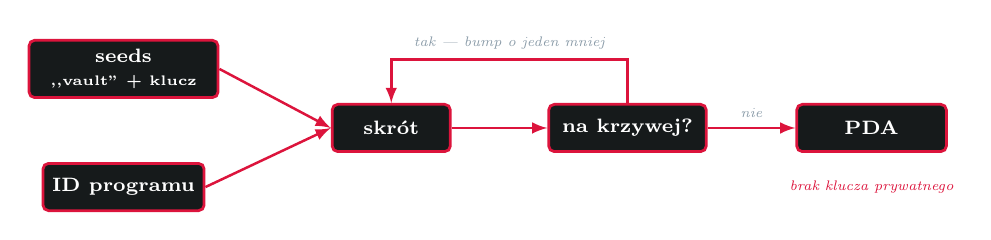
\begin{tikzpicture}[
        every node/.style={font=\scriptsize\bfseries, align=center},
        box/.style={
          draw=stplred, line width=1pt,
          fill=stplcard, text=stplwhite,
          rounded corners=2pt,
          minimum width=1.9cm, minimum height=0.6cm, align=center,
        },
        arr/.style={-latex, draw=stplred, line width=0.9pt},
        lbl/.style={font=\tiny\itshape, text=stplmuted},
      ]
      \node[box, minimum width=2.4cm] (s) at (0, 0) {seeds\\\tiny ,,vault'' + klucz};
      \node[box, minimum width=2.0cm] (p) at (0, -1.5) {ID programu};
      \node[box, minimum width=1.5cm] (h) at (3.4, -0.75) {skrót};
      \node[box, minimum width=2.0cm] (c) at (6.4, -0.75) {na krzywej?};
      \node[box, minimum width=1.9cm] (pda) at (9.5, -0.75) {PDA};

      \draw[arr] (s.east) -- (h.west);
      \draw[arr] (p.east) -- (h.west);
      \draw[arr] (h) -- (c);
      \draw[arr] (c) -- (pda) node[midway, above, lbl] {nie};

      % bump feedback loop
      \draw[arr] (c.north) -- ++(0,0.55) -| (h.north)
        node[pos=0.25, above, lbl] {tak --- bump o jeden mniej};

      \node[lbl, text=stplred] at (9.5, -1.5) {brak klucza prywatnego};
    \end{tikzpicture}
  \end{center}
  \vspace{0.2cm}
  \begin{itemize}
    % Static frame renders overlay 1 only --- explicit <1-> keeps every bullet.
    \item<1-> Ten sam zestaw składników zawsze daje ten sam adres
    \item<1-> Inny program z tymi samymi składnikami dostaje \emph{inny} adres
  \end{itemize}
\end{frame}

% 10. Seeds w Anchorze --- code IS the slide
\begin{frame}[fragile]{Seeds w Anchorze}
  \begin{itemize}
    \item Składniki deklaruje się przy koncie, obok pozostałych constraints
    \item Samo \texttt{bump} bez wartości każe Anchorowi znaleźć bump kanoniczny
    \item Anchor wylicza adres i porównuje go z kontem podanym w transakcji
    \item Niezgodność to błąd \texttt{ConstraintSeeds} --- przed ciałem instrukcji
  \end{itemize}
  \begin{codeblock}{Skarbiec i konto stanu jako PDA}
\begin{lstlisting}[style=reveal]
(*@\onslide<1->@*)#[account(
(*@\onslide<1->@*)    seeds = [LOCKUP_SEED, &payer.key().to_bytes()],
(*@\onslide<2->@*)    bump
(*@\onslide<1->@*))]
(*@\onslide<1->@*)pub locker: Account<'info, Locker>,
(*@\onslide<4->@*)
(*@\onslide<4->@*)// znaleziony bump czeka potem w ctx.bumps.locker
\end{lstlisting}
  \end{codeblock}
\end{frame}

% ================================================================
\section{Podpis PDA}

% 11. Program jako authority --- code IS the slide
\begin{frame}[fragile]{Program podpisuje}
  \begin{itemize}
    \item Authority skarbca to PDA wyprowadzony przez nasz program
    \item Do wywołania dokłada się więc składniki tego PDA razem z bumpem
    \item Zewnętrzna lista to jeden wpis na każdy podpisujący PDA
    \item \texttt{new\_with\_signer} zamiast \texttt{new} --- reszta wywołania bez zmian
  \end{itemize}
  \begin{codeblock}{Wypłata ze skarbca}
\begin{lstlisting}[style=reveal]
(*@\onslide<1->@*)let payer_key = ctx.accounts.payer.key.to_bytes();
(*@\onslide<2->@*)let seeds = &[LOCKUP_SEED, payer_key.as_ref(),
(*@\onslide<2->@*)              &[ctx.bumps.locker]];
(*@\onslide<3->@*)let signer = &[&seeds[..]];
(*@\onslide<4->@*)let cpi_ctx = CpiContext::new_with_signer(
(*@\onslide<4->@*)    ctx.accounts.token_program.key(), cpi_accounts, signer);
(*@\onslide<4->@*)transfer_checked(cpi_ctx, amount, ctx.accounts.mint.decimals)?;
\end{lstlisting}
  \end{codeblock}
\end{frame}

% 12. Kto tu podpisal --- problem hook from the callee's side (alertblock)
\begin{frame}{Kto tu podpisał}
  \begin{itemize}
    \item Token Program dostaje instrukcję i listę kont --- nic więcej
    \item Nie widzi, że między nim a użytkownikiem stoi jakikolwiek program
    \item Nie zna naszych składników, naszego bumpa ani naszej logiki
    \item A jednak musi rozstrzygnąć, czy przelew jest autoryzowany
  \end{itemize}
  \vspace{0.25cm}
  \begin{alertblock}{Pytanie}
    Skąd wywoływany program wie, że wolno mu ruszyć cudze saldo ---
    skoro nie dostał żadnego podpisu do sprawdzenia?
  \end{alertblock}
\end{frame}

% 13. Propagacja --- choreographed TikZ synced to bullets (§4.5b).
%     This is the only frame that states the mechanism; the prose version that
%     used to sit here said the same four things in words.
\begin{frame}{Podpis się przenosi}
  \begin{center}
    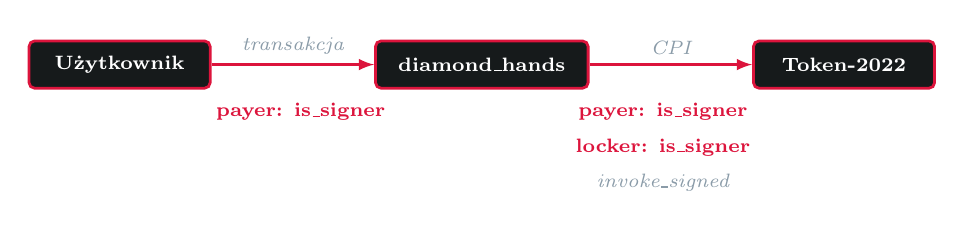
\begin{tikzpicture}[
        every node/.style={font=\scriptsize\bfseries, align=center},
        box/.style={
          draw=stplred, line width=1pt,
          fill=stplcard, text=stplwhite,
          rounded corners=2pt,
          minimum width=2.3cm, minimum height=0.6cm, align=center,
        },
        arr/.style={-latex, draw=stplred, line width=0.9pt},
        lbl/.style={font=\scriptsize\itshape, text=stplmuted},
        flag/.style={font=\scriptsize\bfseries, text=stplred},
      ]
      % Stage 1: the three participants + the outer transaction
      \node[box] (u) at (0, 0) {Użytkownik};
      \node[box, minimum width=2.7cm] (d) at (4.6, 0) {diamond\_hands};
      \node[box, minimum width=2.3cm] (t) at (9.2, 0) {Token-2022};
      \draw[arr] (u) -- (d) node[midway, above, lbl] {transakcja};

      % Stage 2: the user's flag, set once at the transaction boundary
      \begin{scope}[visible on=<2->]
        \node[flag] at (2.3, -0.6) {payer: is\_signer};
      \end{scope}

      % Stage 3: the CPI hop --- the same flag travels
      \begin{scope}[visible on=<3->]
        \draw[arr] (d) -- (t) node[midway, above, lbl] {CPI};
        \node[flag] at (6.9, -0.6) {payer: is\_signer};
      \end{scope}

      % Stage 4: invoke_signed adds a second flag
      \begin{scope}[visible on=<4->]
        \node[flag] at (6.9, -1.05) {locker: is\_signer};
        \node[lbl] at (6.9, -1.5) {invoke\_signed};
      \end{scope}
    \end{tikzpicture}
  \end{center}
  \vspace{-0.3cm}
  \begin{itemize}
    \item<+-> Sieć weryfikuje podpis użytkownika \textbf{raz}, przy transakcji
    \item<+-> Flaga \texttt{is\_signer} zostaje na koncie \texttt{payer}
    \item<+-> Przy CPI flaga przechodzi do wywołania niezmieniona
    \item<+-> \texttt{invoke\_signed} dokłada drugą --- dla PDA \texttt{locker}
  \end{itemize}
  \begin{block}{Kluczowe zdanie}
    Przy podpisie PDA nie powstaje żaden podpis kryptograficzny --- wywoływany
    traktuje konto tak, jakby było podpisane.
    \hfill\textcolor{stplmuted}{\tiny docs.rs/solana-cpi}
  \end{block}
\end{frame}

% 14. Sprawdzenie u wywolywanego --- code IS the slide (the payoff)
\begin{frame}[fragile]{Sprawdzenie u odbiorcy}
  \begin{itemize}
    \item Token Program porównuje podane authority z zapisanym w koncie
    \item Potem sprawdza jedną flagę --- i na tym cała weryfikacja się kończy
    \item Nie pyta, czy flagę postawił człowiek, czy program
    \item Ta sama linia obsługuje podpis użytkownika i podpis PDA
  \end{itemize}
  \begin{codeblock}{Weryfikacja po stronie Token Programu}
\begin{lstlisting}[style=reveal]
(*@\onslide<1->@*)if expected_owner != owner_account_info.key {
(*@\onslide<1->@*)    return Err(TokenError::OwnerMismatch.into());
(*@\onslide<1->@*)}
(*@\onslide<2->@*)if !owner_account_info.is_signer {
(*@\onslide<2->@*)    return Err(ProgramError::MissingRequiredSignature);
(*@\onslide<2->@*)}
(*@\onslide<4->@*)// flaga is_signer to jedyna informacja o autoryzacji
\end{lstlisting}
  \end{codeblock}
\end{frame}

% 15. Dwa zrodla flagi --- A-vs-B opposition (§4.4, no helper block)
\begin{frame}{Dwa źródła flagi}
  % Both columns open with a block, whose leading \pause would push the first
  % bullet past overlay 1 and open the frame on a blank slide.
  \addtocounter{beamerpauses}{-3}%
  \begin{columns}
    \column{0.48\textwidth}
      \begin{block}{Podpis użytkownika}
        \begin{itemize}
          \item<+-> Dowodem jest \textbf{klucz prywatny}
          \item<+-> Wystawia go człowiek, poza łańcuchem
          \item<+-> Sięga po środki właściciela klucza
          \item<+-> Wyciek klucza to utrata środków
        \end{itemize}
      \end{block}

    \column{0.48\textwidth}
      \begin{alertblock}{Podpis PDA}
        \begin{itemize}
          \item<+-> Dowodem jest \textbf{kod programu}
          \item<+-> Wystawia go program, w trakcie wykonania
          \item<+-> Sięga wyłącznie po własne PDA
          \item<+-> Nie ma czego wykraść --- jest co audytować
        \end{itemize}
      \end{alertblock}
  \end{columns}
  \vspace{0.15cm}
  \begin{center}
    \textcolor{stplmuted}{\small Dla odbiorcy obie flagi wyglądają identycznie ---
    a CPI potrafi uprawnienia wyłącznie \textbf{zawężać}.}
  \end{center}
\end{frame}

% ================================================================
\section{Podsumowanie}

% 17. Pulapki --- (alertblock: risks)
\begin{frame}{Pułapki}
  \begin{itemize}
    \item Składniki bez klucza użytkownika dają \textbf{jeden wspólny PDA}
    \item Bump przyjęty od klienta pozwala trafić w adres inny niż kanoniczny
    \item Podpis PDA autoryzuje wywołanie --- nie zastępuje kontroli, kto o nie prosi
  \end{itemize}
  \vspace{0.1cm}
  \begin{center}
    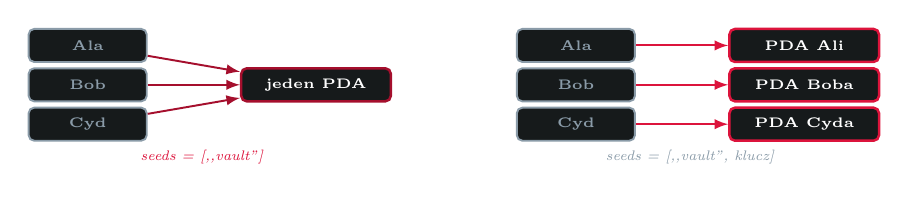
\begin{tikzpicture}[
        every node/.style={font=\tiny\bfseries, align=center},
        u/.style={
          draw=stplmuted, line width=0.7pt,
          fill=stplcard, text=stplmuted,
          rounded corners=2pt,
          minimum width=1.5cm, minimum height=0.42cm, align=center,
        },
        pda/.style={
          draw=stplred, line width=0.9pt,
          fill=stplcard, text=stplwhite,
          rounded corners=2pt,
          minimum width=1.9cm, minimum height=0.42cm, align=center,
        },
        arr/.style={-latex, draw=stplred, line width=0.7pt},
        lbl/.style={font=\tiny\itshape, text=stplmuted},
      ]
      % BAD: one shared PDA
      \node[u] (a1) at (0, 0.5) {Ala};
      \node[u] (b1) at (0, 0.0)  {Bob};
      \node[u] (c1) at (0,-0.5) {Cyd};
      \node[pda, draw=stplred!75!black] (s) at (2.9, 0) {jeden PDA};
      \draw[arr, draw=stplred!75!black] (a1) -- (s);
      \draw[arr, draw=stplred!75!black] (b1) -- (s);
      \draw[arr, draw=stplred!75!black] (c1) -- (s);
      \node[lbl, text=stplred] at (1.45, -0.92) {seeds = [,,vault'']};

      % GOOD: one PDA per user
      \node[u] (a2) at (6.2, 0.5) {Ala};
      \node[u] (b2) at (6.2, 0.0)  {Bob};
      \node[u] (c2) at (6.2,-0.5) {Cyd};
      \node[pda] (p1) at (9.1, 0.5) {PDA Ali};
      \node[pda] (p2) at (9.1, 0.0)  {PDA Boba};
      \node[pda] (p3) at (9.1,-0.5) {PDA Cyda};
      \draw[arr] (a2) -- (p1);
      \draw[arr] (b2) -- (p2);
      \draw[arr] (c2) -- (p3);
      \node[lbl] at (7.65, -0.92) {seeds = [,,vault'', klucz]};
    \end{tikzpicture}
  \end{center}
  \vspace{0.05cm}
  \begin{alertblock}{Zasada}
    Podpis PDA mówi wyłącznie ,,ten program się zgadza''.
    Czy zgodzić się \emph{powinien}, sprawdza sam program --- constraints i \texttt{Signer}.
  \end{alertblock}
\end{frame}

\begin{frame}{Podsumowanie}
  \begin{enumerate}
    \item \textbf{CPI} to wywołanie innego programu wewnątrz jednej transakcji
    \item \textbf{PDA} to adres wyliczony ze składników i ID programu, bez klucza
    \item \textbf{Bump} przesuwa skrót poza krzywą --- kanoniczny to pierwszy trafiony
    \item Flaga \texttt{is\_signer} \textbf{przenosi się} w dół drzewa wywołań
    \item Odbiorca sprawdza samą flagę --- i to wystarcza mu za dowód tożsamości
  \end{enumerate}
  \vspace{0.2cm}
  \begin{exampleblock}{Efekt}
    Podpis PDA to sposób, w jaki jeden program dowodzi drugiemu swojej
    tożsamości --- bez klucza, bez podpisu, na jednej fladze.
  \end{exampleblock}
\end{frame}

% ================================================================
\begin{frame}[plain]
  \begin{center}
    \vfill
    {\Huge\bfseries\color{stplwhite} gn}
    \vfill
  \end{center}
\end{frame}

\end{document}
